\documentclass[11pt,a4paper]{article}

% ---------------------------------------------------------------- packages
\usepackage[T1]{fontenc}
\usepackage[utf8]{inputenc}
\usepackage{mathpazo}                 % Palatino text and maths
\usepackage[scaled=0.92]{helvet}      % sans-serif for headings
\usepackage{amsmath,amssymb,bm}
\usepackage[a4paper,margin=2.3cm,headheight=14pt]{geometry}
\usepackage{microtype}
\usepackage{graphicx}
\usepackage{booktabs,tabularx}
\usepackage[table]{xcolor}
\usepackage{titlesec}
\usepackage{fancyhdr}
\usepackage{enumitem}
\usepackage{caption,subcaption}
\usepackage[most]{tcolorbox}
\usepackage{listings}
\usepackage[section]{placeins}   % keep figures inside their section
\usepackage[hidelinks]{hyperref}

% ---------------------------------------------------------------- design
\definecolor{ink}{HTML}{1F2A33}
\definecolor{accent}{HTML}{0B6E8A}
\definecolor{soft}{HTML}{E8F3F6}
\definecolor{codebg}{HTML}{F6F7F8}

\titleformat{\section}{\sffamily\Large\bfseries\color{accent}}{\thesection}{0.8em}{}[\vspace{-0.4ex}{\color{accent}\titlerule[0.6pt]}]
\titleformat{\subsection}{\sffamily\large\bfseries\color{ink}}{\thesubsection}{0.7em}{}
\titleformat{\paragraph}[runin]{\sffamily\bfseries\color{ink}}{}{}{}[.]
\titlespacing*{\section}{0pt}{3.2ex}{1.6ex}

\pagestyle{fancy}
\fancyhf{}
\renewcommand{\headrulewidth}{0pt}
\fancyhead[L]{\sffamily\footnotesize\color{accent} Visual Servoing \& Image-Space Planning}
\fancyhead[R]{\sffamily\footnotesize\color{accent} D26027}
\fancyfoot[C]{\sffamily\footnotesize\thepage}

\captionsetup{font=small,labelfont={sf,bf,color=accent},labelsep=period}
\setlist{itemsep=2pt,topsep=4pt}
\renewcommand{\arraystretch}{1.18}
\setlength{\emergencystretch}{3em}

\lstset{basicstyle=\ttfamily\footnotesize,backgroundcolor=\color{codebg},frame=single,
        rulecolor=\color{codebg},xleftmargin=4pt,xrightmargin=4pt,aboveskip=6pt,belowskip=6pt,
        keywordstyle=\color{accent}\bfseries,commentstyle=\color{gray},language=Python,
        columns=fullflexible,keepspaces=true}

\newtcolorbox{keybox}[1]{enhanced,colback=soft,colframe=accent,boxrule=0pt,leftrule=3pt,
  arc=0pt,outer arc=0pt,left=8pt,right=8pt,top=5pt,bottom=5pt,
  title={\sffamily\bfseries #1},coltitle=accent,attach title to upper,after title={\par\smallskip}}

\newcommand{\vect}[1]{\bm{#1}}
\newcommand{\pinv}{^{+}}

% ================================================================ document
\begin{document}

% ---------------------------------------------------------------- title block
\thispagestyle{empty}
\begin{tcolorbox}[enhanced,colback=accent,colframe=accent,arc=0pt,outer arc=0pt,
                  left=14pt,right=14pt,top=14pt,bottom=12pt,width=\textwidth]
  {\color{white}\sffamily
   {\small ASSIGNMENT 3 \;\textbar\; AR523 ROBOT MANIPULATORS}\\[6pt]
   {\LARGE\bfseries Image-Based Visual Servoing and\\[2pt] Image-Space RRT/RRT$^{*}$ for a UR5}\\[10pt]
   {\normalsize Deepak Singh Gariya \;\textbullet\; Roll No.\ D26027 \;\textbullet\; November 2026}}
\end{tcolorbox}

\vspace{4pt}
\noindent\textbf{\sffamily\color{accent}Abstract.}\;
A camera on the tool of a simulated UR5 must make a target appear at a chosen position and size in
its image. I implemented image-based visual servoing with a $3\times6$ interaction matrix for the
target's centroid and area, extended it to a target moving on a circle by estimating and cancelling
the target's motion, and avoided an obstacle by planning in image space with RRT and RRT$^{*}$ whose
nodes also carry the robot configuration. On top of this baseline I added four improvements: an
adaptive gain, a two-step-ahead prediction of the target's motion, shortcutting of the planned path,
and a final IBVS stage after the plan. Together they halve the time Task~1 needs to reach 10\,px
(5.9\,s to 3.0\,s), cut the moving-target tracking error from 9.0\,px to 0.43\,px, and bring the final
error of the planning tasks from 62--95\,px down to 1\,px, with no collision in any run.


\begin{keybox}{Results at a glance ($\vect s^{*}=[40,\,30,\,2500]$)}
\small
\begin{tabularx}{\linewidth}{@{}lXrr@{}}
  & & \textbf{Baseline} & \textbf{Improved}\\
  Task 1 & time to reach 10\,px & 5.9\,s & 3.0\,s\\
  Task 2 & steady tracking error (compensated) & 9.0\,px & 0.43\,px\\
  Task 3 & final error to $\vect s^{*}$ (classic IBVS collides in both) & 61.9\,px & 1.0\,px\\
  Task 4 & final error to $\vect s^{*}$; RRT$^{*}$ path 4.4$\times$ shorter than RRT & 94.6\,px & 1.0\,px\\
  All & collisions & 0 & 0
\end{tabularx}
\end{keybox}


% ---------------------------------------------------------------- 1
\section{Introduction}

A camera is fixed to the tool of a simulated UR5 arm. The goal is to move the arm until a small
coloured box appears in the camera image at a chosen place and with a chosen size. The arm is never
told a position in metres: it is steered only by what the camera sees. This is image-based visual
servoing (IBVS) \cite{chaumette2006}.

The assignment has four tasks. Task~1 servos to a static target, Task~2 tracks a target moving on a
circle, and Tasks~3--4 add an obstacle that plain IBVS drives into, which is solved by planning a path
in image space with RRT and then RRT$^{*}$. I first implemented the nine required parts (TODO~0 to
TODO~8, Sections~\ref{sec:setup}--\ref{sec:baseline}). I then added four improvements of my own
(Section~\ref{sec:improvements}), each of which can be switched off in
\texttt{config/experiment\_config.py} to get back to the baseline.

% ---------------------------------------------------------------- 2
\section{Problem setup}\label{sec:setup}

\paragraph{Camera and features} The camera image is $640\times480$\,px with focal length
$f_x=f_y=500$\,px. The simulator segments the target by colour, giving a binary region $\mathcal{D}$,
and summarises it by three numbers computed from image moments \cite{chaumette2004}:
\begin{equation}
  \vect{s}=\begin{bmatrix}x_c & y_c & a\end{bmatrix}^{\!\top},\qquad
  a=m_{00},\quad x_c=\frac{m_{10}}{m_{00}},\quad y_c=\frac{m_{01}}{m_{00}},\qquad
  m_{ij}=\sum_{(x,y)\in\mathcal{D}} x^{i}y^{j}.
\end{equation}
Here $(x_c,y_c)$ is the centre of the target in pixels, measured from the image centre ($x$ to the
right, $y$ down), and $a$ is the number of pixels it covers. A nearer camera sees a bigger target:
for a target of fixed size, $a\propto 1/Z^{2}$, where $Z$ is the camera--target distance.

\paragraph{Desired feature (TODO~0)} I chose
\begin{equation}
  \vect{s}^{*}=\begin{bmatrix}40 & 30 & 2500\end{bmatrix}^{\!\top},
\end{equation}
which puts the target slightly right of and below the image centre with an area of 2500\,px$^{2}$.
All three values sit inside the recommended ranges ($0\le x^{*}\le100$, $0\le y^{*}\le80$,
$2000\le a^{*}\le3000$), so the goal is reachable in every task. The start view in Tasks~1--2 is
$\vect{s}_0=[156.5,\,-122.8,\,1450]^{\top}$: the target starts up and to the right, and smaller,
so the camera has to move towards it.

\paragraph{Error and control loop} The error is $\vect{e}=\vect{s}-\vect{s}^{*}$. Every
$\Delta t=0.1$\,s the controller measures $\vect{s}$, computes a camera twist
$\vect{v}_c=[v_x,v_y,v_z,\omega_x,\omega_y,\omega_z]^{\top}$ in the camera frame, converts it to joint
rates with the camera Jacobian, $\dot{\vect q}=J_c\pinv\vect{v}_c$, scales them down if any joint would
exceed its speed limit (3.15\,rad/s), and moves the arm. Only the step from $\vect{e}$ to $\vect{v}_c$
is designed in this assignment.

% ---------------------------------------------------------------- 3
\section{Method}\label{sec:method}

\subsection{Interaction matrix (TODO 1)}

The interaction matrix $L$ tells how fast each feature changes when the camera moves:
\begin{equation}
  \dot{\vect{s}}=L(\vect{s},Z)\,\vect{v}_c,\qquad L\in\mathbb{R}^{3\times6}.
\end{equation}
For a point at depth $Z$ with normalised coordinates $x=X/Z$, $y=Y/Z$, a static point moves relative
to the camera as $\dot{\vect P}=-\vect v-\vect\omega\times\vect P$. Differentiating the projection gives
the classical point rows \cite{chaumette2006}:
\begin{align}
  L_x&=\begin{bmatrix}-\tfrac1Z & 0 & \tfrac xZ & xy & -(1+x^{2}) & y\end{bmatrix},\\
  L_y&=\begin{bmatrix}0 & -\tfrac1Z & \tfrac yZ & 1+y^{2} & -xy & -x\end{bmatrix}.
\end{align}
The entries have a direct meaning. The $-1/Z$ in the $v_x$ column says that moving the camera to the
right makes the target slide left in the image, and faster when it is close. The $x/Z$ in the $v_z$
column says that approaching the target spreads points away from the image centre. The rotation
columns do not depend on $Z$: turning the camera shifts near and far points alike.

For the area, $a\propto1/Z^{2}$ gives $\dot a/a=-2\dot Z/Z$; moving forward at $v_z$ means
$\dot Z=-v_z$, so $\dot a=(2a/Z)\,v_z$. For a planar target parallel to the image plane the full row
from the moment-based derivation \cite{chaumette2004} is
\begin{equation}
  L_a=\begin{bmatrix}0 & 0 & \tfrac{2a}{Z} & 3ay & -3ax & 0\end{bmatrix}.
\end{equation}
The features are in pixels, $x_c=f_x x$, so the first row is multiplied by $f_x$ and the second by
$f_y$; the area is already in px$^{2}$ and its row is used as it is:
$L=\begin{bmatrix}f_xL_x;\ f_yL_y;\ L_a\end{bmatrix}$.
\begin{lstlisting}
x, y = xc / fx, yc / fy                       # pixels -> normalised
L_x = fx * np.array([-1/Z, 0, x/Z, x*y, -(1 + x**2), y])
L_y = fy * np.array([0, -1/Z, y/Z, 1 + y**2, -x*y, -x])
L_a = np.array([0, 0, 2*a/Z, 3*a*y, -3*a*x, 0])
return np.array([L_x, L_y, L_a])
\end{lstlisting}
As a check, $\vect s=[100,-50,1000]$ and $Z=0.5$ give $x=0.2$, $y=-0.1$ and a first row
$500\cdot[-2,0,0.4,-0.02,-1.04,-0.1]=[-1000,0,200,-10,-520,-50]$, exactly the value the unit test
expects.

\subsection{Classic IBVS law (TODO 2)}

The design goal is an error that shrinks by the same fraction every second, without overshoot:
\begin{equation}
  \dot{\vect e}=-\lambda\vect e\quad\Longrightarrow\quad \vect e(t)=\vect e(0)\,e^{-\lambda t}.
\end{equation}
For a static target $\dot{\vect e}=L\vect v_c$. Setting $L\vect v_c=-\lambda\vect e$ requires inverting $L$,
which is $3\times6$ and has no inverse. The Moore--Penrose pseudo-inverse $L\pinv=L^{\top}(LL^{\top})^{-1}$
gives the smallest twist that produces the wanted error rate:
\begin{equation}\label{eq:ibvs}
  \vect v_c=-\lambda\,L\pinv\vect e,\qquad \lambda=1\ \text{s}^{-1}.
\end{equation}
The code uses the provided damped pseudo-inverse, which replaces each $1/\sigma_i$ by
$\sigma_i/(\sigma_i^{2}+\delta^{2})$ and so stays bounded near singular poses.

\subsection{Moving target (TODOs 3 and 4)}

When the target moves, the error changes for two reasons, the camera's motion and the target's own:
\begin{equation}
  \dot{\vect e}=L\vect v_c+\frac{\partial\vect e}{\partial t}.
\end{equation}
The classic law only reacts to error that already exists, so it always trails the target. The
target's part cannot be measured directly, but it is what remains of the measured feature rate once
the part caused by the camera's last command is removed (TODO~3):
\begin{equation}\label{eq:motion}
  \widehat{\frac{\partial\vect e}{\partial t}}=\frac{\vect s_k-\vect s_{k-1}}{\Delta t}-L_{k-1}\vect v_{k-1}.
\end{equation}
The provided loop smooths this estimate with a first-order filter of weight $\alpha=0.5$. Asking again
for $\dot{\vect e}=-\lambda\vect e$ and solving for $\vect v_c$ gives the compensated law (TODO~4):
\begin{equation}\label{eq:comp}
  \vect v_c=-L\pinv\!\left(\lambda\vect e+\widehat{\frac{\partial\vect e}{\partial t}}\right).
\end{equation}
The extra term is a feed-forward: the camera follows the target's motion as it happens instead of
waiting for an error to build up.

\subsection{Image-space RRT (TODOs 5 and 6)}

IBVS is greedy: each step reduces the image error as fast as possible and ignores everything else, so
with an obstacle between the start and goal poses it drives straight into it. The fix is to plan
first. The planner grows two coupled trees, one of features $\vect s$ and one of configurations
$\vect q$; each feature node stores the configuration that produces it. Because every node has a real
$\vect q$, each node and each edge is checked for field of view, occlusion by the obstacle, collision
(with a 2\,cm safety margin) and joint limits.

Each iteration samples $\vect s_{\text{rand}}$ (the goal every 10th time, otherwise a feature from a
dataset of 2000 views the robot can produce), finds the nearest node, and extends it by one step
(TODO~5):
\begin{align}
  \dot{\vect s}&=\lambda_{\text{RRT}}\,(\vect s_{\text{rand}}-\vect s_{\text{parent}}),\qquad \lambda_{\text{RRT}}=0.5,\\
  J_1&=L(\vect s_{\text{parent}},Z)\,J_c(\vect q_{\text{parent}}),\\
  \dot{\vect q}&=J_1\pinv\dot{\vect s}+P_1(J_2P_1)\pinv\!\left(\vect 0-J_2J_1\pinv\dot{\vect s}\right),\qquad P_1=I-J_1\pinv J_1,\\
  \vect q_{\text{new}}&=\vect q_{\text{parent}}+\dot{\vect q}\,\Delta t_{\text{RRT}},\qquad \Delta t_{\text{RRT}}=1\ \text{s}.
\end{align}
$J_1$ maps joint rates straight to feature rates. The image task uses only three of the six joint
freedoms; the other three are used by a secondary task, $J_2=J_c[3{:}6,:]$, that keeps the camera
orientation fixed. Projecting it through $P_1$ means it never disturbs the image task. Planning stops
at the first node within 75\,px of $\vect s^{*}$. TODO~6 draws the result: grey parent--child edges,
blue nodes and the start-to-goal path in red, both in the 3-D feature space and in the image plane.

The robot then follows the planned features $\vect s^{*}_k$ with trajectory-tracking IBVS. This is the
law of Eq.~\eqref{eq:comp} with the plan's own velocity in the role of the target's motion, which is why
Task~2 comes before Task~3:
\begin{equation}
  \vect v_c=-\lambda L\pinv(\vect s_k-\vect s^{*}_k)+L\pinv\,\frac{\vect s^{*}_k-\vect s^{*}_{k-1}}{\Delta t}.
\end{equation}

\subsection{Image-space RRT$^{*}$ (TODOs 7 and 8)}

RRT attaches each new node to whichever node is nearest to the random sample and stops at the first
solution, so its paths wander. RRT$^{*}$ \cite{karaman2011} keeps a cost $c(i)$ for every node, the
length of its path back to the root in feature space, and adds two steps for each new node, using the
neighbours $\mathcal N$ within 150\,px:
\begin{itemize}
  \item \textbf{Choose parent (TODO 7).} Connect the new node to
        $\arg\min_{i\in\mathcal N}\, c(i)+\lVert\vect s_{\text{new}}-\vect s_i\rVert$, among the
        neighbours that a valid edge can reach (at most 0.5\,rad of joint motion, collision-free,
        target visible). The cost comparison is done first, since the edge check is expensive.
  \item \textbf{Rewire (TODO 8).} For each neighbour $j$, if
        $c(\text{new})+\lVert\vect s_j-\vect s_{\text{new}}\rVert<c(j)$ and the edge is valid, make the
        new node the parent of $j$ in \emph{both} trees and lower the cost of $j$ and its whole subtree by
        the same amount. A loop cannot form: if $j$ were an ancestor of the new node, the new node's cost
        would already be at least $c(j)$.
\end{itemize}
RRT$^{*}$ does not stop at the first solution: it runs all 3000 iterations and returns the cheapest node
within the goal radius.

% ---------------------------------------------------------------- 4
\section{Baseline results}\label{sec:baseline}

Table~\ref{tab:baseline} lists the results with only the TODOs implemented. All 37 unit tests pass.

\begin{table}[htbp]
\centering\small
\caption{Baseline results (TODOs 0--8 only).}\label{tab:baseline}
\begin{tabular}{@{}clr@{}}
\toprule
Task & Measure & Value\\
\midrule
1 & feature error, start $\rightarrow$ end of 10\,s & 1067\,px $\rightarrow$ 0.006\,px\\
1 & time to reach 10\,px & 5.9\,s\\
2 & steady tracking error, classic / compensated & 57.2\,px / 9.0\,px\\
2 & largest steady error, classic / compensated & 74.5\,px / 11.3\,px\\
3 & classic IBVS (no planning) & collision after 3 steps\\
3 & RRT: iterations / nodes / path cost & 280 / 74 / 3283\\
3 & final error / mean tracking error & 61.9\,px / 20.6\,px\\
3 & collisions / smallest clearance & 0 / 2.98\,cm\\
4 & path cost RRT / RRT$^{*}$ & 5848 / 1340\\
4 & planning time RRT / RRT$^{*}$ & 5.0\,s / 8.7\,s\\
4 & final error / mean tracking error & 94.6\,px / 27.0\,px\\
4 & collisions / smallest clearance & 0 / 2.25\,cm\\
\bottomrule
\end{tabular}
\end{table}

\paragraph{Task 1} The error falls on a straight line in a log plot (Fig.~\ref{fig:base12}a), which is
the signature of exponential decay, from 1067\,px down to a few pixels. Below that it jumps between 0
and 2\,px, because the centroid is computed from whole pixels and the camera cannot see smaller
errors. The target crosses the image in an almost straight line, a known property of IBVS.

\paragraph{Task 2} The classic law settles into a constant lag, its error swinging between 35 and
75\,px as the target circles. Compensation removes most of it (9.0\,px), and the estimated target rate
is a clean pair of sine waves with the 8\,s period of the circle (Fig.~\ref{fig:base12}b).

\begin{figure}[htbp]
\centering
\begin{subfigure}{0.49\linewidth}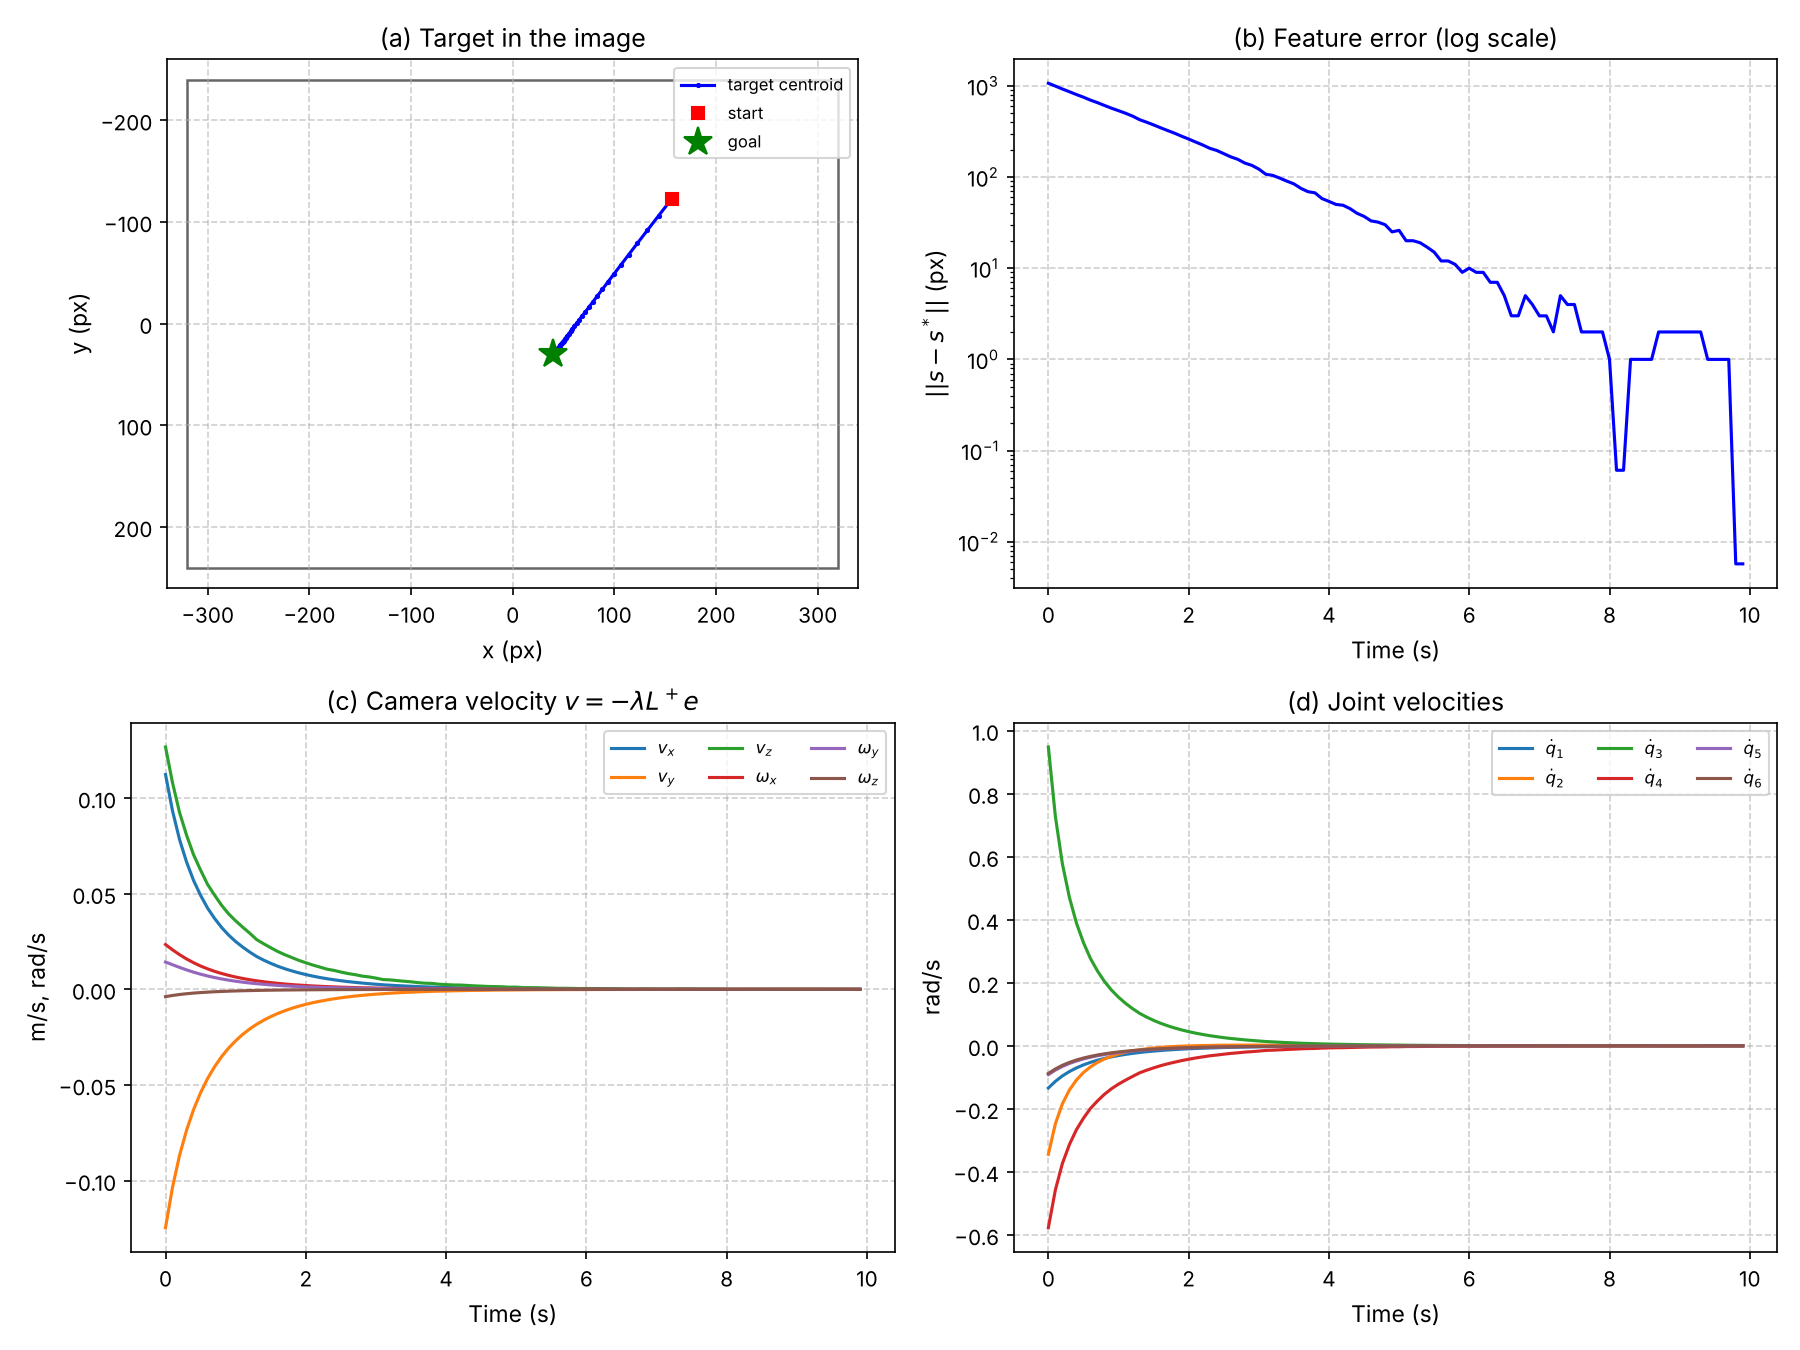
\includegraphics[width=\linewidth]{figures/task1_baseline.png}\caption{Task 1}\end{subfigure}\hfill
\begin{subfigure}{0.49\linewidth}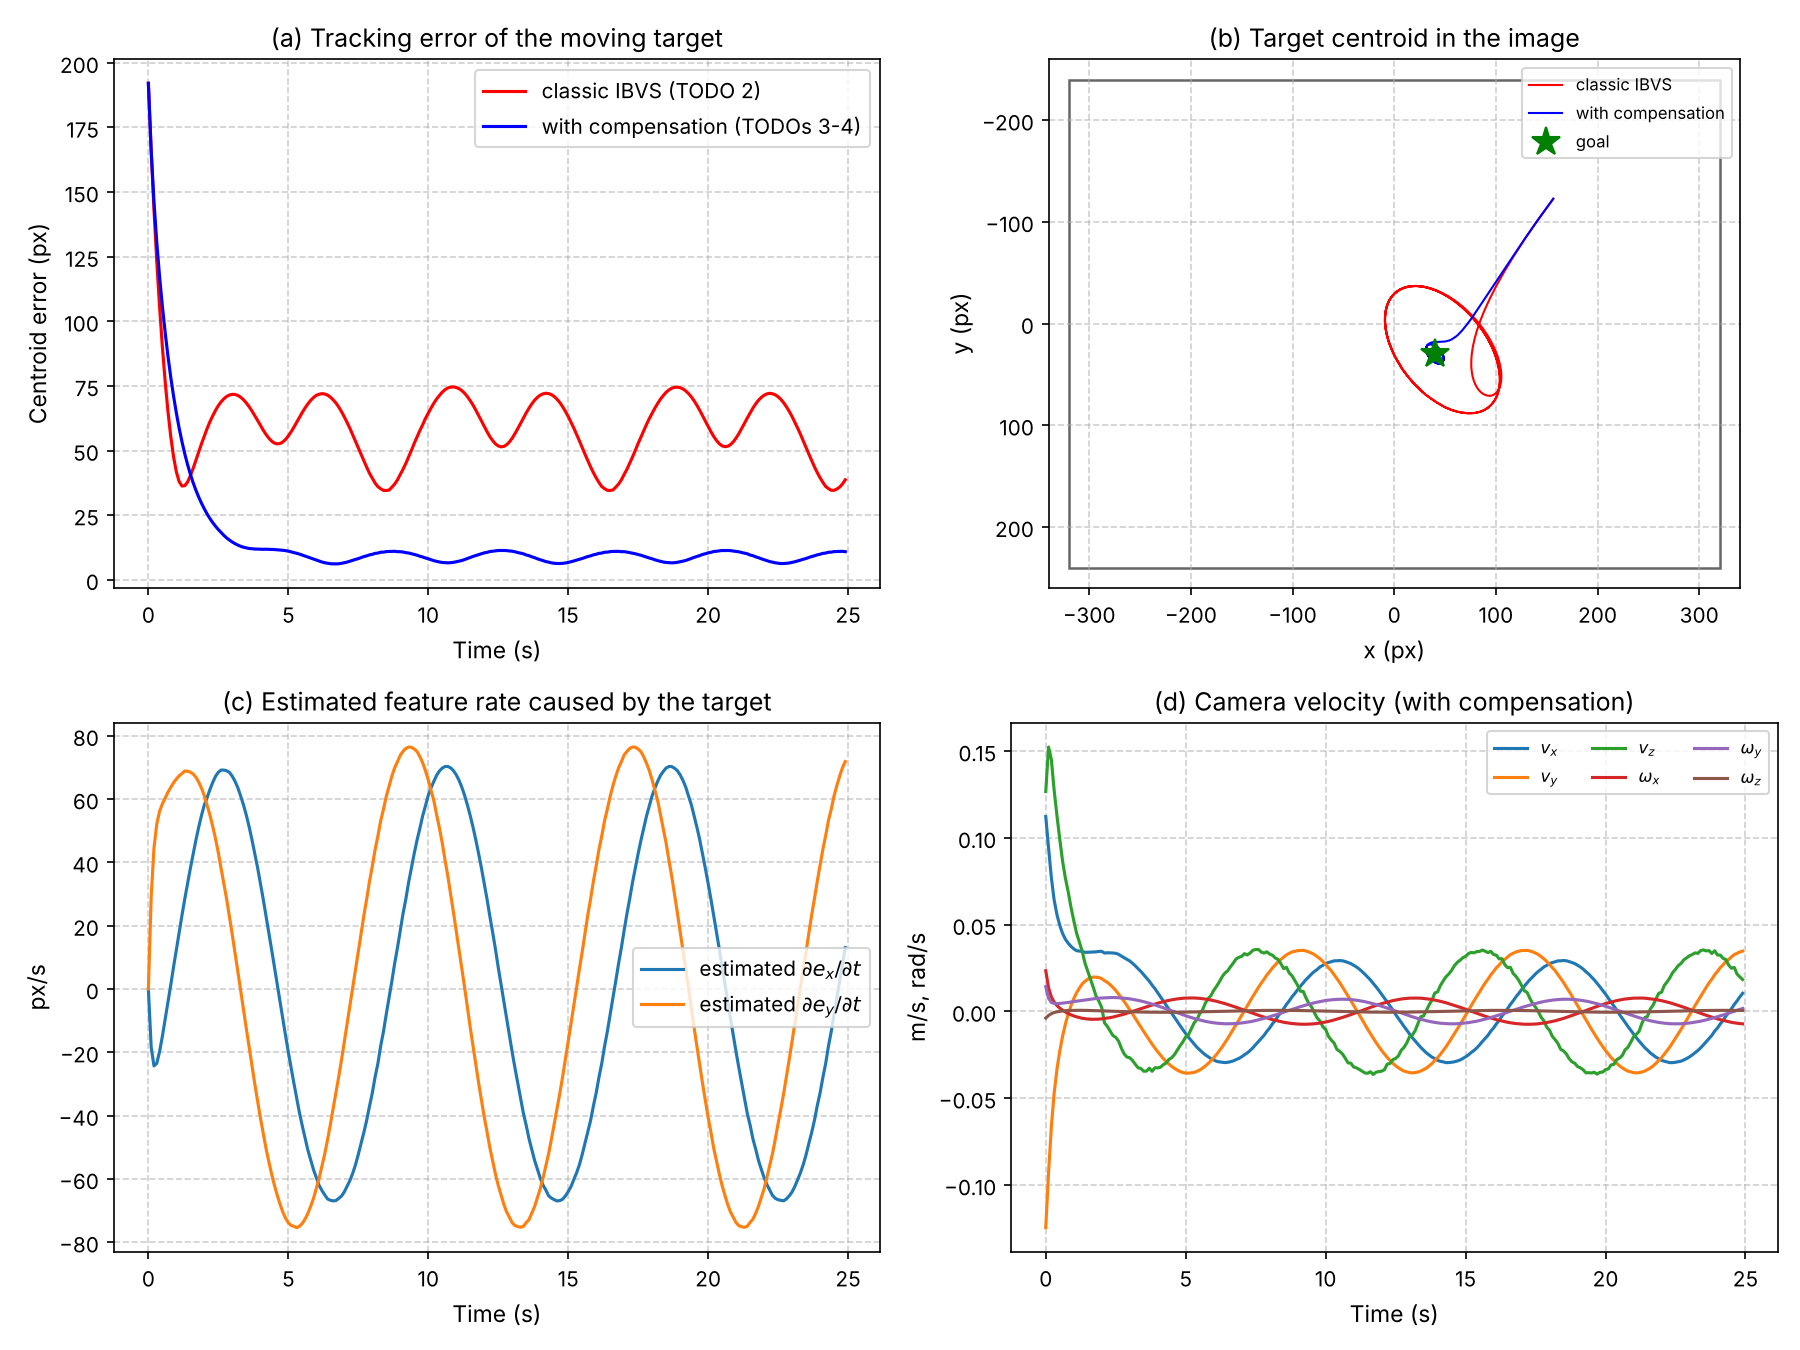
\includegraphics[width=\linewidth]{figures/task2_baseline.png}\caption{Task 2}\end{subfigure}
\caption{Baseline IBVS. (a) Target path in the image, error on a log scale, camera twist and joint
rates. (b) Tracking error of classic (red) and compensated (blue) IBVS, the target's path in the
image, the estimated target rate and the camera twist.}\label{fig:base12}
\end{figure}

\paragraph{Tasks 3 and 4} Classic IBVS hits the pillar after 3 steps (Fig.~\ref{fig:task3}, top row).
The RRT path goes around it with zero collisions, but it ends 62\,px from $\vect s^{*}$, and in
Task~4 the RRT$^{*}$ path ends 95\,px away. This is the main weakness of the baseline: the planner stops
as soon as a node is within 75\,px of the goal, and the tracking controller stops at the last waypoint,
so nothing ever drives the camera the rest of the way.

\begin{figure}[htbp]
\centering
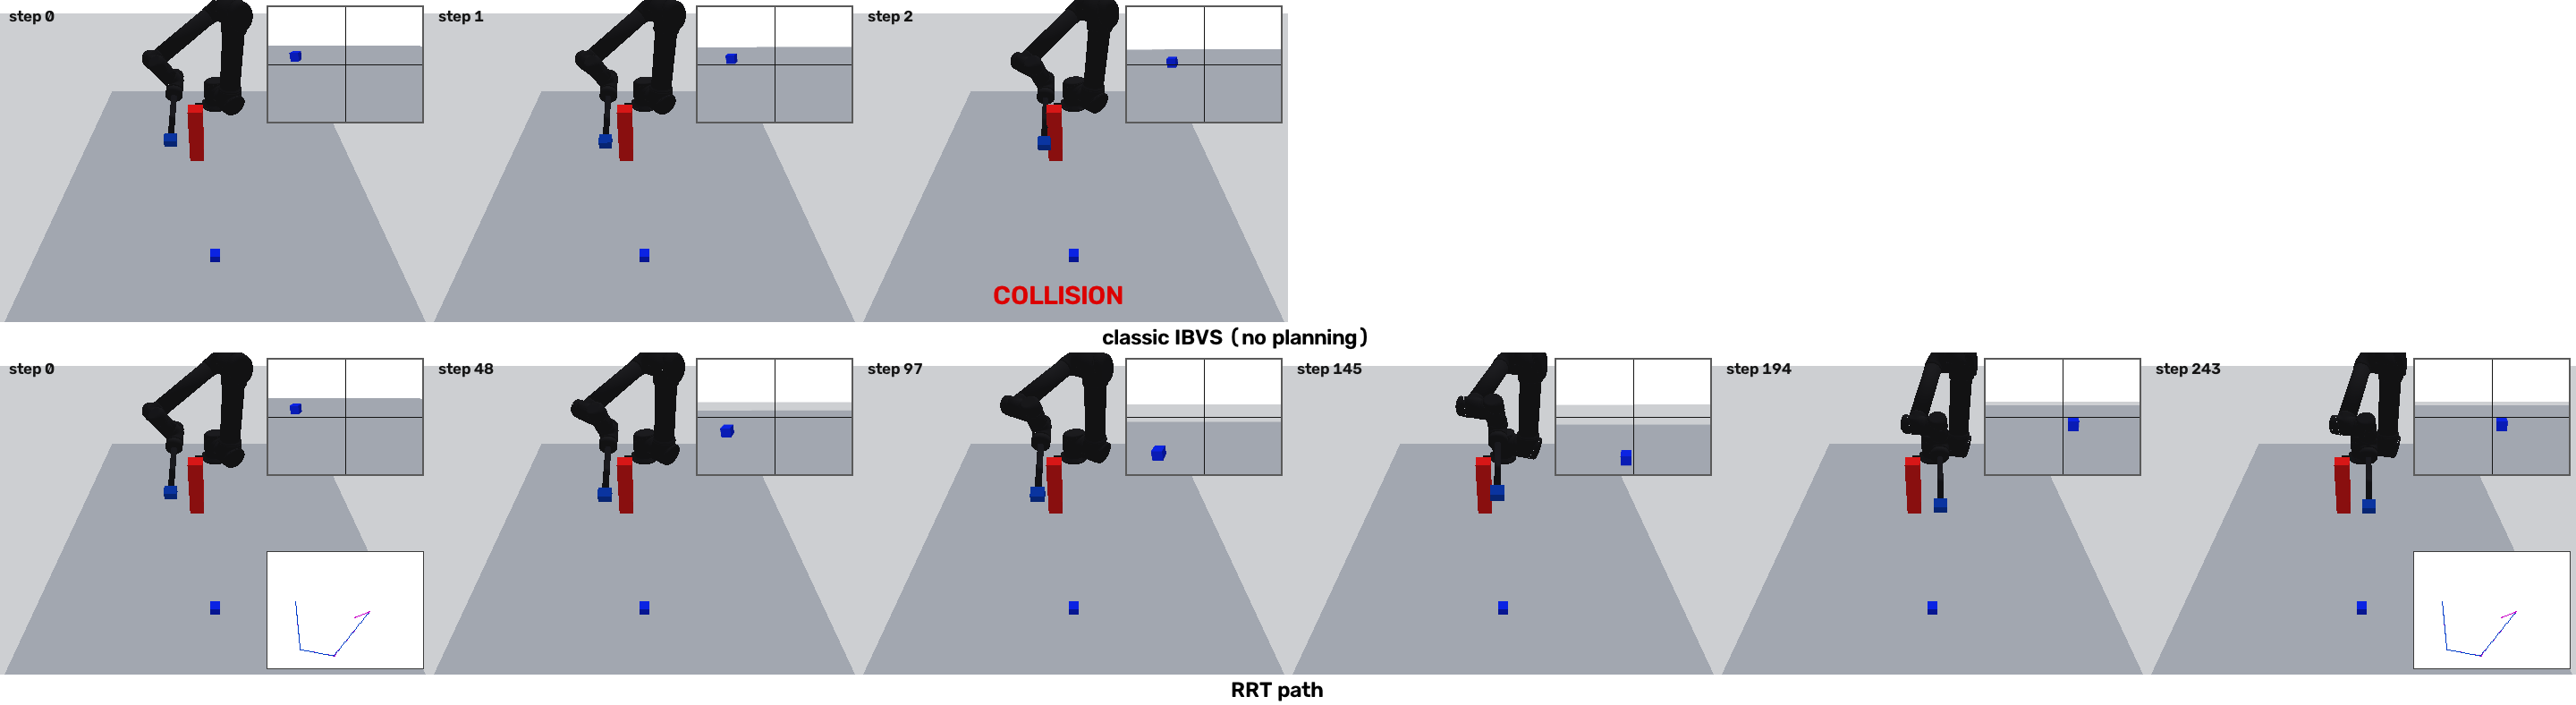
\includegraphics[width=\linewidth]{figures/task3_motion_sequence.png}
\caption{Task 3. Top: classic IBVS drives into the red pillar. Bottom: the robot following the planned
path around it; the insets show the camera view and the planned path in the image.}\label{fig:task3}
\end{figure}

% ---------------------------------------------------------------- 5
\section{Improvements}\label{sec:improvements}

Each improvement targets one weakness seen above, and each has an on/off switch in
\texttt{config/experiment\_config.py}. With all four switches off, the code reproduces the baseline
numbers exactly.
\begin{center}\small
\begin{tabular}{@{}lll@{}}
\toprule
Improvement & Switch & Tasks\\
\midrule
Adaptive gain & \texttt{USE\_ADAPTIVE\_GAIN} & 1, 2\\
Target-motion prediction & \texttt{USE\_MOTION\_PREDICTION} & 2\\
Path shortcutting & \texttt{USE\_PATH\_SHORTCUT} & 3, 4\\
Final IBVS stage & \texttt{USE\_FINAL\_IBVS} & 3, 4\\
\bottomrule
\end{tabular}
\end{center}

\subsection{Adaptive gain (Tasks 1--2)}

A fixed $\lambda$ is a compromise. A large gain gives large velocities when the error is large, and a
small gain makes the last part of the motion slow, because the error shrinks by the same fraction each
second however small it already is. I used the adaptive gain of ViSP \cite{visp2005}, which is low
far from the goal and rises as the error gets small:
\begin{equation}
  \lambda(\lVert\vect e\rVert)=(\lambda_0-\lambda_\infty)\exp\!\left(-\frac{\lambda'_0\,\lVert\vect e\rVert}{\lambda_0-\lambda_\infty}\right)+\lambda_\infty,
  \qquad \lambda_0=4,\ \lambda_\infty=1\ \text{s}^{-1},\ \lambda'_0=0.015\ \text{s}^{-1}\text{px}^{-1}.
\end{equation}
At the start ($\lVert\vect e\rVert\approx1000$\,px) the gain is 1.0, exactly the baseline, so the largest
joint speed is unchanged (0.96 against 0.95\,rad/s). At 100\,px it is 2.8 and near zero error it is 4.
I tuned $\lambda'_0$ by trying 0.015--0.04: smaller slopes raise the gain earlier and reached 10\,px
fastest. With $\lambda\Delta t\le0.4$ the discrete loop stays far from its stability limit of 2.

\subsection{Target-motion prediction (Task 2)}

The remaining 9\,px in Task~2 is a lag. The estimate of Eq.~\eqref{eq:motion} is built from the
\emph{previous} interval and then smoothed, while the command acts over the \emph{next} interval, so the
camera always uses a target velocity about one and a half steps old. On a circle that velocity keeps
turning, so an old value points the wrong way. A rough check confirms the size: the target's image
speed is about 70\,px/s and turns at $2\pi/8=0.79$\,rad/s, so 1.5 steps of delay is a direction error of
0.12\,rad, a velocity error of about 8\,px/s, and with $\lambda=1$ a steady error of about 8\,px.

I therefore also estimate how fast the target-motion estimate itself is changing, its trend
$\vect r$, and use the value predicted $H$ steps ahead, as in an $\alpha$--$\beta$ tracking filter
\cite{barshalom2001}:
\begin{equation}
  \vect r_k=(1-\beta)\,\vect r_{k-1}+\beta\,\frac{\hat{\vect d}_k-\hat{\vect d}_{k-1}}{\Delta t},\qquad
  \hat{\vect d}^{\,\text{pred}}_k=\hat{\vect d}_k+H\Delta t\,\vect r_k,\qquad \beta=0.5,\ H=2,
\end{equation}
where $\hat{\vect d}_k$ is the filtered estimate of $\partial\vect e/\partial t$. The prediction
replaces $\hat{\vect d}_k$ in Eq.~\eqref{eq:comp}. I chose $\beta$ and $H$ by trying $\beta\in\{0.2,0.3,0.5\}$
and $H\in\{1,2,3\}$: on its own, with a fixed gain, the best setting lowered the steady error from 9.0
to 1.4\,px; $H=3$ over-predicts and is worse again.

\subsection{Path shortcutting (Tasks 3--4)}

A random tree reaches the goal through detours. After planning, I shorten the path greedily
\cite{geraerts2007}: from the current node, try to jump straight to the \emph{last} node of the path,
then to the one before it, and so on, and keep the first jump that is valid. A jump is valid if it
needs at most 1.0\,rad of motion in every joint and every configuration along the straight joint-space
edge, checked every 0.05\,rad, keeps the target in view, is not hidden by the obstacle and keeps the
2\,cm margin. The same checks as the planner's own edges are used, so the shortened path is as safe as
the original. Path costs in Section~\ref{sec:improved} are reported both for the tree and for the
shortened path, so the RRT against RRT$^{*}$ comparison stays fair.

\subsection{Final IBVS stage (Tasks 3--4)}

When the last waypoint is reached the camera is past the obstacle and within the planner's goal radius
of $\vect s^{*}$. From there the remaining motion is a short, unobstructed servoing problem, so the
controller switches to plain IBVS towards $\vect s^{*}$, still holding the camera orientation fixed
through the same secondary task:
\begin{equation}
  \dot{\vect q}=J_1\pinv(-\lambda_f\vect e)+P_1(J_2P_1)\pinv\!\left(\vect 0-J_2J_1\pinv(-\lambda_f\vect e)\right),\qquad \lambda_f=1.5\ \text{s}^{-1}.
\end{equation}
It runs until $\lVert\vect e\rVert<1.5$\,px, for at most 80 steps, and stops early if the next pose would
enter the 2\,cm safety margin around the obstacle.

% ---------------------------------------------------------------- 6
\section{Results with the improvements}\label{sec:improved}

Every task improved where it was weakest, and no run collided (Table~\ref{tab:improved},
Fig.~\ref{fig:cmp}). The two planning tasks now end within 1\,px of $\vect s^{*}$ instead of 62 and
95\,px, at the cost of 2--6\,s of extra motion for the final stage.

\begin{table}[htbp]
\centering\small
\caption{Baseline against improved. Unit tests: 37 of 37 pass in both configurations.}\label{tab:improved}
\begin{tabular}{@{}clrr@{}}
\toprule
Task & Measure & Baseline & Improved\\
\midrule
1 & time to reach 10\,px & 5.9\,s & \textbf{3.0\,s}\\
1 & final error & 0.006\,px & 0.006\,px\\
1 & largest joint speed & 0.95\,rad/s & 0.96\,rad/s\\
\midrule
2 & steady error, classic IBVS & 57.2\,px & 39.1\,px\\
2 & steady error, compensated & 9.0\,px & \textbf{0.43\,px}\\
2 & largest steady error, compensated & 11.3\,px & \textbf{0.59\,px}\\
\midrule
3 & classic IBVS (no planning) & collision, 3 steps & collision, 2 steps\\
3 & path cost (tree / executed) & 3283 / 3283 & 3283 / \textbf{2624}\\
3 & nodes on the path & 11 & 4\\
3 & error when the plan ends & 61.9\,px & 81.8\,px\\
3 & final error & 61.9\,px & \textbf{1.0\,px}\\
3 & motion time (plan + final stage) & 22.5\,s & 17.7 + 6.7 = 24.4\,s\\
3 & collisions / smallest clearance & 0 / 2.98\,cm & 0 / 2.20\,cm\\
\midrule
4 & RRT path cost (tree / executed) & 5848 / 5848 & 5848 / \textbf{2161}\\
4 & RRT$^{*}$ path cost (tree / executed) & 1340 / 1340 & 1340 / \textbf{1306}\\
4 & error when the plan ends & 94.6\,px & 50.8\,px\\
4 & final error & 94.6\,px & \textbf{1.0\,px}\\
4 & motion time (plan + final stage) & 9.4\,s & 9.0 + 6.1 = 15.1\,s\\
4 & collisions / smallest clearance & 0 / 2.25\,cm & 0 / 2.33\,cm\\
\bottomrule
\end{tabular}
\end{table}

\begin{figure}[htbp]
\centering
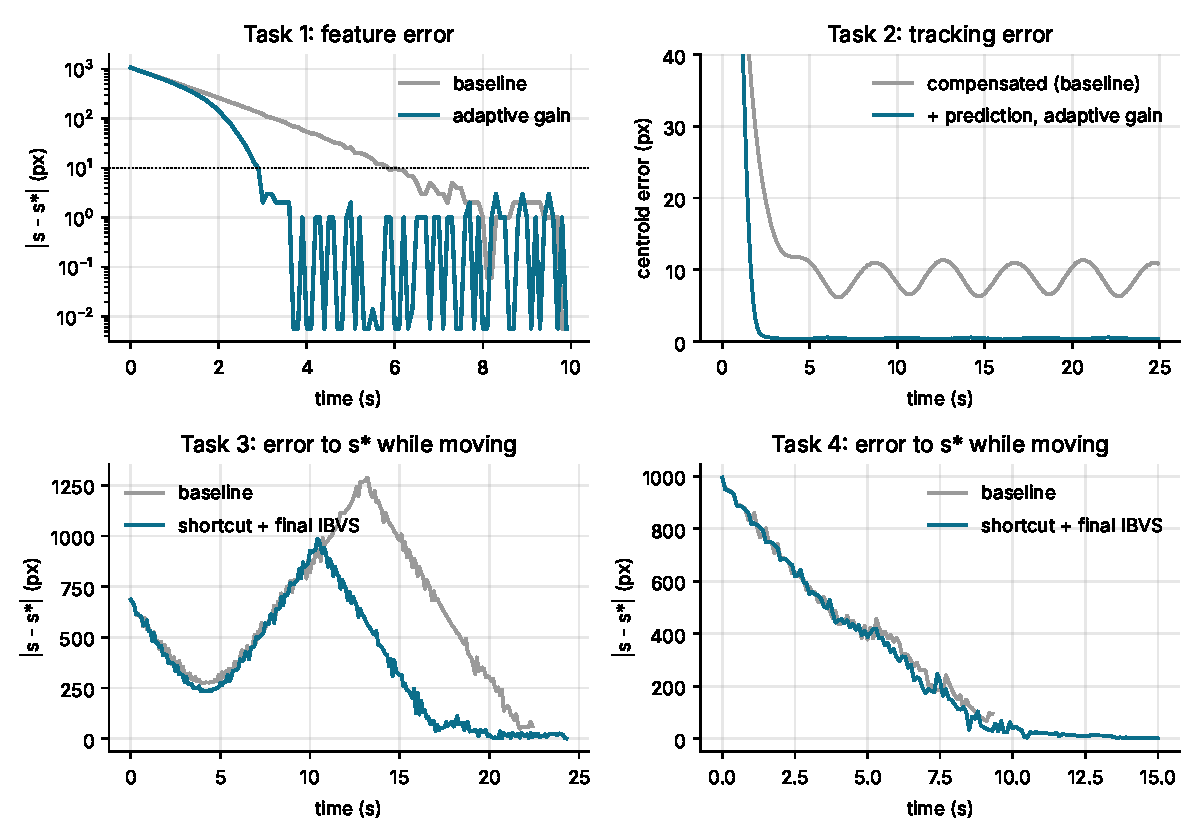
\includegraphics[width=0.9\linewidth]{figures/comparison.pdf}
\caption{Baseline (grey) against improved (blue). Task 1: the adaptive gain reaches 10\,px (dotted)
in half the time. Task 2: prediction and the adaptive gain remove the oscillating lag. Tasks 3--4:
the shortened path ends sooner and the final IBVS stage then takes the error to 1\,px.}\label{fig:cmp}
\end{figure}

\begin{figure}[htbp]
\centering
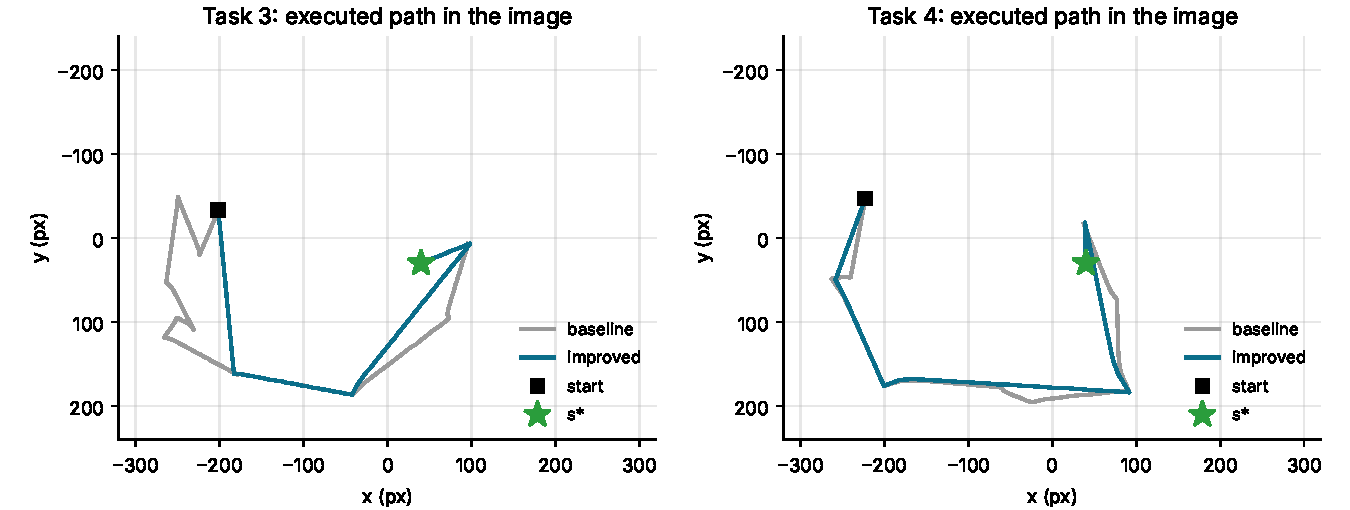
\includegraphics[width=0.92\linewidth]{figures/paths.pdf}
\caption{Executed paths of the target in the image. Shortcutting removes the zig-zags of the random tree;
the final stage adds the short last segment into $\vect s^{*}$.}\label{fig:paths}
\end{figure}

\begin{figure}[htbp]
\centering
\begin{subfigure}{0.49\linewidth}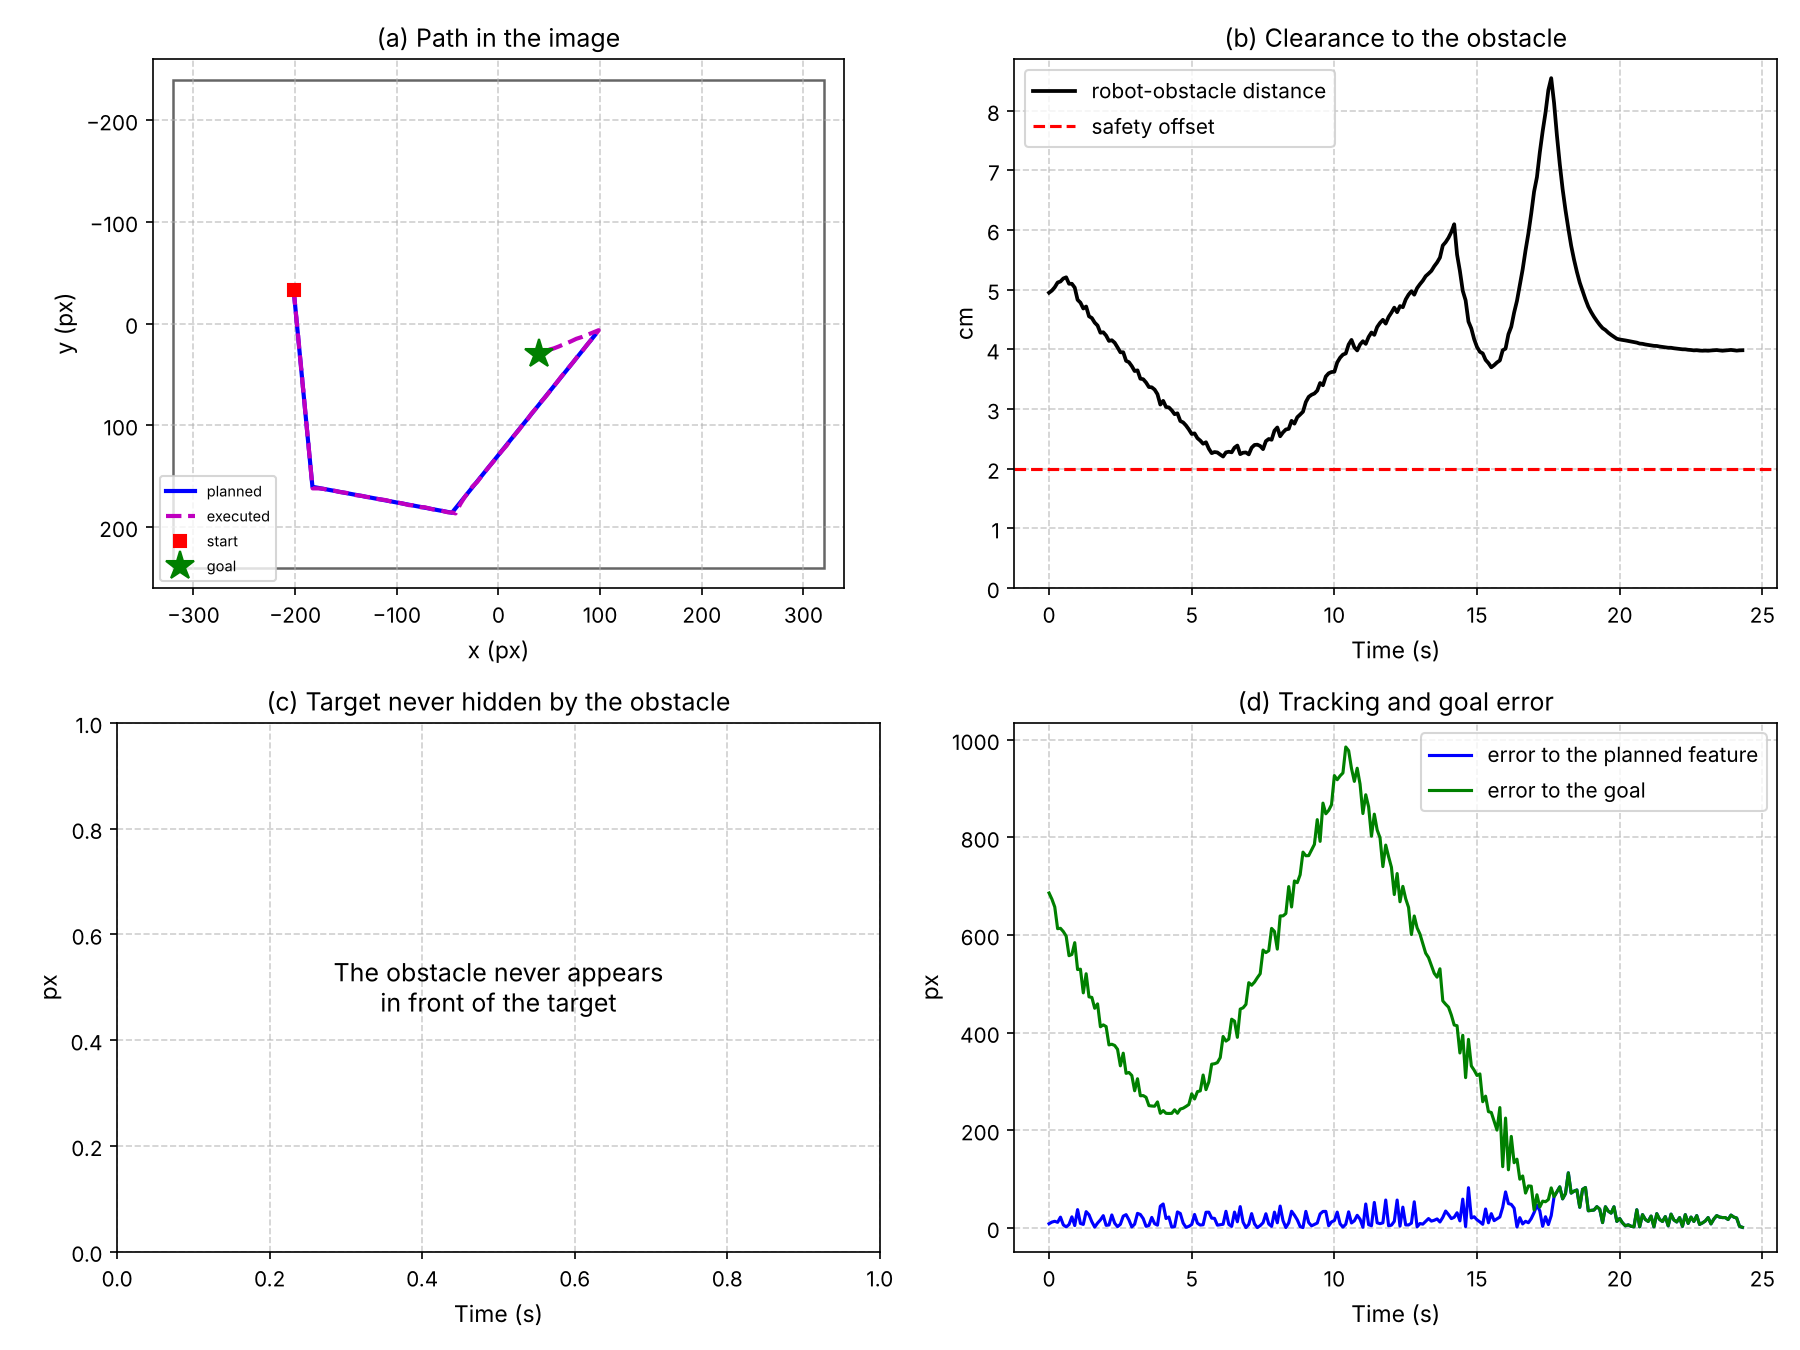
\includegraphics[width=\linewidth]{figures/task3_improved.png}\caption{Task 3}\end{subfigure}\hfill
\begin{subfigure}{0.49\linewidth}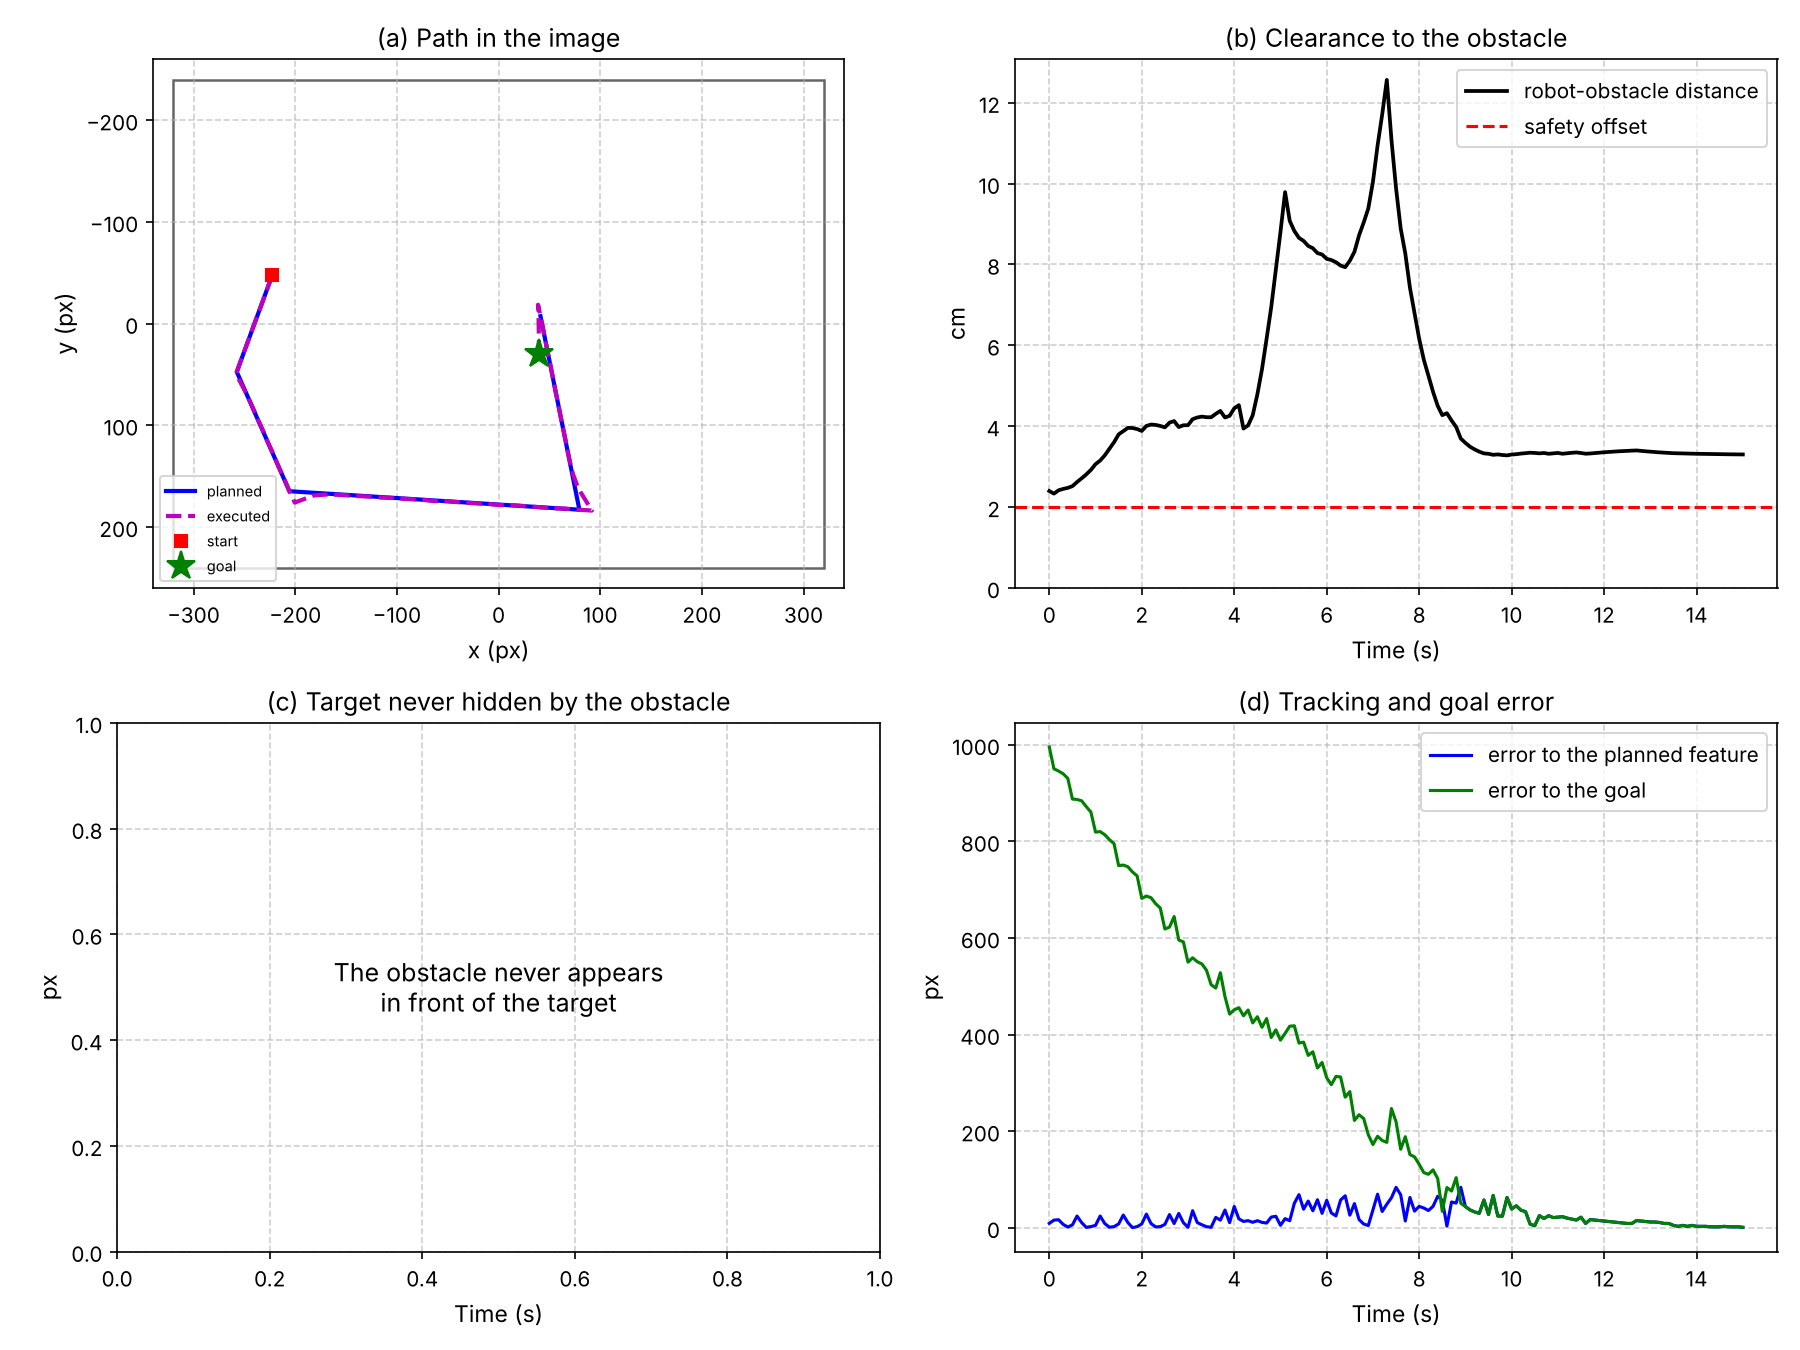
\includegraphics[width=\linewidth]{figures/task4_improved.png}\caption{Task 4}\end{subfigure}
\caption{Executions with the improvements: path in the image, clearance to the obstacle (dashed line:
2\,cm margin), occlusion check, and tracking and goal error.}\label{fig:imp34}
\end{figure}

\begin{figure}[htbp]
\centering
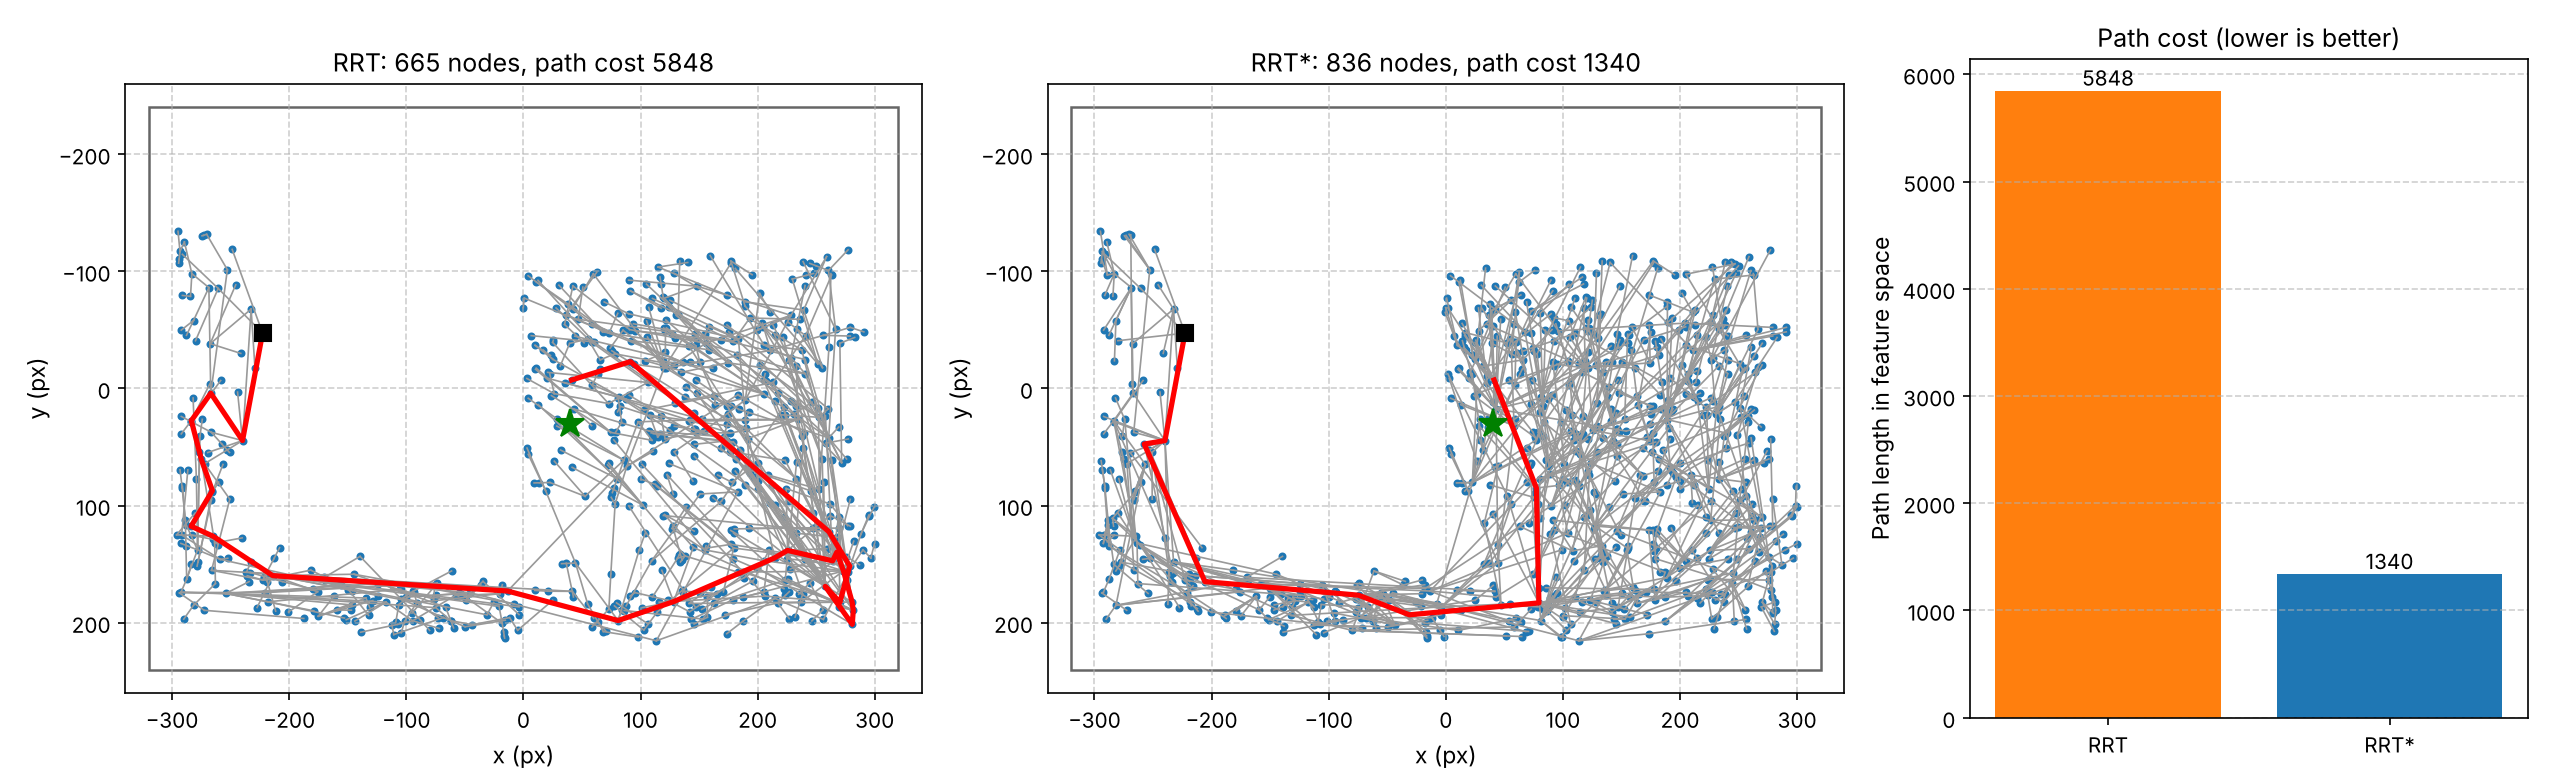
\includegraphics[width=\linewidth]{figures/task4_rrt_vs_rrt_star.png}
\caption{Task 4 trees: RRT (left) and RRT$^{*}$ (middle) with the chosen path in red, and the tree path
costs (right).}\label{fig:rrtstar}
\end{figure}

% ---------------------------------------------------------------- 7
\section{Discussion}

\paragraph{The final stage matters most for Tasks 3--4} It took the final error from 62 and 95\,px to
1\,px in 67 and 61 extra steps. The clearance during the final stage stayed above 3.3\,cm in both
tasks, so the safety stop was never needed. This confirms the idea behind it: the planner only has to
get the camera safely past the obstacle; the last few centimetres are an ordinary IBVS problem.

\paragraph{Shortcutting helps RRT far more than RRT$^{*}$} It cut the RRT path in Task~4 by 63\,\%
(5848 to 2161) but the RRT$^{*}$ path by only 2.5\,\% (1340 to 1306), because RRT$^{*}$ has already
removed most detours during planning by rewiring. RRT$^{*}$ is still the shorter of the two after
shortcutting, by a factor of 1.65. Shortcutting can only delete nodes from a path that exists;
RRT$^{*}$ can find a different, better route.

\paragraph{Motion time} The improved runs take longer in Task~4 (9.4 to 15.1\,s) and slightly longer in
Task~3 (22.5 to 24.4\,s). The planned motion itself got shorter (17.7 and 9.0\,s), but the final stage
adds about 6--7\,s, because its error decays exponentially from 50--80\,px down to 1.5\,px with
$\lambda_f=1.5$. A higher $\lambda_f$, or the adaptive gain applied to the final stage, would shorten
this; the trade-off is speed against how gently the arm approaches its final pose.

\paragraph{Precision near the goal} In Task~1 the adaptive gain reaches 10\,px in 3.0\,s, but afterwards
the error hops between 0 and 1\,px (Fig.~\ref{fig:cmp}) instead of settling smoothly. With a gain of 4
near the goal, each one-pixel jump in the measured centroid produces a visible correction. The final
error is the same 0.006\,px as the baseline.

\paragraph{Task 2 prediction is tuned to smooth motion} The trend term assumes the target's image
velocity changes smoothly, which is exactly true for a circle. For a target that stops or turns
sharply the prediction would overshoot for a few steps. The adaptive gain also helped classic IBVS
(57 to 39\,px) because it raises the gain once the error is small, but the lag of classic IBVS is
structural and only compensation removes it.

\paragraph{Limitations} The area row of $L$ assumes a target parallel to the image plane, while in
Tasks~3--4 the camera looks down at 20$^{\circ}$; the feedback corrects the resulting model error. The
depth $Z$ is taken from the simulator; a real system would have to estimate it, for example from the
measured area. Shortcut edges are checked as straight lines in joint space, while the controller tracks
straight lines in feature space between waypoints, so the executed motion can differ slightly from the
checked edge; the smallest clearance, 2.2\,cm, stayed above the 2\,cm margin in every run.

% ---------------------------------------------------------------- 8
\section{Conclusion}

All nine required parts work: classic IBVS converges exponentially, the compensated law tracks a moving
target six times better than classic IBVS, and image-space RRT and RRT$^{*}$ avoid the obstacle that
makes IBVS alone fail, RRT$^{*}$ with a 4.4 times shorter path. The four improvements address the weak
points this left. The adaptive gain halves the time to converge, predicting the target's motion cuts
the tracking error by a factor of 20 to 0.43\,px, and path shortcutting with a final IBVS stage brings
the camera to within 1\,px of $\vect s^{*}$ in the planning tasks, without any collision.

\paragraph{Reproducing the results} The code is in the repository
\url{https://github.com/deepakgariaa/visual-servoing}, branch
\texttt{claude/festive-brown-ws92ga}.
Running \texttt{python main.py --all --headless} reproduces the improved results; setting the four
\texttt{USE\_*} switches to \texttt{False} reproduces the baseline. Running
\texttt{python report/make\_figures.py} redraws the comparison figures.


% ---------------------------------------------------------------- references
\begin{thebibliography}{9}\small
\bibitem{chaumette2006} F.~Chaumette and S.~Hutchinson, ``Visual servo control, Part I: Basic approaches,''
  \emph{IEEE Robotics \& Automation Magazine}, vol.~13, no.~4, pp.~82--90, 2006.
\bibitem{chaumette2004} F.~Chaumette, ``Image moments: a general and useful set of features for visual servoing,''
  \emph{IEEE Transactions on Robotics}, vol.~20, no.~4, pp.~713--723, 2004.
\bibitem{lavalle1998} S.~M.~LaValle, ``Rapidly-exploring random trees: a new tool for path planning,''
  Technical Report 98-11, Iowa State University, 1998.
\bibitem{karaman2011} S.~Karaman and E.~Frazzoli, ``Sampling-based algorithms for optimal motion planning,''
  \emph{International Journal of Robotics Research}, vol.~30, no.~7, pp.~846--894, 2011.
\bibitem{visp2005} E.~Marchand, F.~Spindler and F.~Chaumette, ``ViSP for visual servoing: a generic software
  platform with a wide class of robot control skills,'' \emph{IEEE Robotics \& Automation Magazine},
  vol.~12, no.~4, pp.~40--52, 2005.
\bibitem{barshalom2001} Y.~Bar-Shalom, X.~R.~Li and T.~Kirubarajan, \emph{Estimation with Applications to
  Tracking and Navigation}. Wiley, 2001.
\bibitem{geraerts2007} R.~Geraerts and M.~H.~Overmars, ``Creating high-quality paths for motion planning,''
  \emph{International Journal of Robotics Research}, vol.~26, no.~8, pp.~845--863, 2007.
\bibitem{corke2017} P.~Corke, \emph{Robotics, Vision and Control}, 2nd ed. Springer, 2017.
\end{thebibliography}

\end{document}
